\section{Постановка задачи}

По смоделированным выборкам из нормального распределения с произвольными математическими ожиданиями $a_x$, $a_y$ и произвольными дисперсиями $\sigma^2_x$, $\sigma^2_y$ необходимо проверить гипотезу о независимости номинальных признаков, используя 2 статистики

\begin{equation}\label{x}
	X^2 = \sum\limits_{i=1}^r \sum\limits_{j=1}^s \frac{\left(n_{ij} - \frac{n_i m_j}{n}\right)^2}{\frac{n_i m_j}{n}}
\end{equation}

\begin{equation}\label{y}
	Y^2 = 2 \sum\limits_{i=1}^r \sum\limits_{j=1}^s n_{ij} \ln \left(\frac{n_{ij}}{\frac{n_i m_j}{n}}\right),
\end{equation}
где 

\begin{equation*}
	n_i = \sum\limits_{j=1}^s n_{ij}; 
\end{equation*}

\begin{equation*}
	m_j = \sum\limits_{i=1}^r n_{ij};
\end{equation*}

\begin{equation*}
	n = \sum\limits_{i=1}^r \sum\limits_{j=1}^s n_{ij};
\end{equation*}

\section{Ход работы}

Были сгенерированы выборки объёмом $n = 200$ из нормального распределения (параметры и сами выборки находятся в конце файла). Поле наблюдений представлено на графике снизу.

\begin{figure}[H]
	\begin{minipage}[H]{0.9\linewidth}
		\begin{center}
			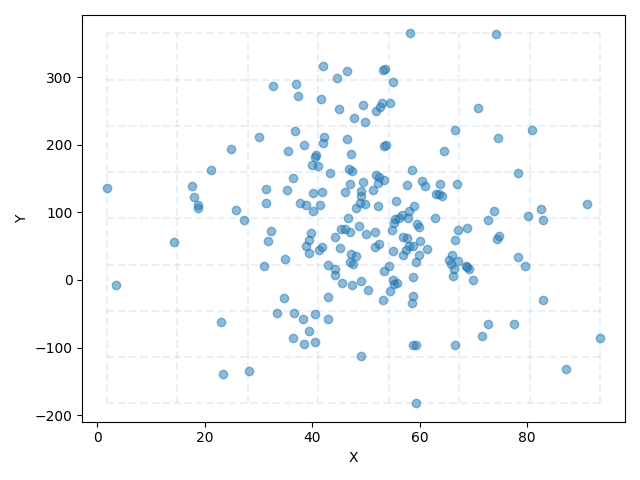
\includegraphics[width=\linewidth]{figures/scatters}
		\end{center}
	\end{minipage}
\end{figure}

Можно разбить ось $x$ на $r$ непересекающихся промежутков, а ось $y$ -- на $s$ промежутков. В результате можно считать, что имеется два номинальных признака -- признак $A$ имеет $r$ уровней $A_1, \ldots, A_r$; признак $B$ имеет $s$ уровней $B_1, \ldots, B_s$. Таким образом, имеется выборка случайно отобранных $n$ объектов из генеральной совокупности, по которой нужно найти частоты совместной встречаемости событий $A_i \cap B_j$.

Частоты собираются в таблицу, называемую таблицей сопряжённости. Ниже такая таблица сформирована по моделированным выше выборкам

\VerbatimInput{figures/table.txt}

Таблица численно показывает распределение наблюдений, которые изображены на графике.

Пусть $p_{ij} = P(A_i \cup B_j)$, $p_i = P(A_i)$, $q_j = P(B_j)$. Сформулируем гипотезу о независимости признаков $A$ и $B$: $H_0: p_{ij} = p_i q_j$, $i=\overline{1,r}$, $j = \overline{1, s}$. При этом $p_i = \sum\limits_{j=1}^s p_{ij}$, $q_i = \sum\limits_{i=1}^r p_{ij}$

Метод проверки гипотезы $H_0$ основан на статистиках (\ref{x}) и (\ref{y}). Если признаки $A$ и $B$ независимы, то статистики $X^2$ и $Y^2$ имеют распределение $\chi^2$ с $(r - 1)(s - 1)$ степенями свободы.

Таким образом,

\begin{itemize}
	\item Для независимых признаков статистика $X^2$ асимптотически распределена по закону $\chi^2$ с $(r - 1)(s - 1)$ степенями свободы.
	\item Для зависимых признаков $X^2$ неограниченно возрастает при увеличениии $n$
\end{itemize}

Для проверки гипотезы необходимо вычислить одну из статистик (\ref{x}) и (\ref{y}) и сравнить их с соответствующими критическими значениями $\chi^2_{\alpha}$ -- верхняя квантиль уровня $\alpha$ из распределения $\chi^2$ с $(r - 1)(s - 1)$ степенями свободы.

Гипотеза $H_0$
\begin{itemize}
	\item Принимается, если $X^2 < \chi^2_{\alpha}$ ($Y^2 < \chi^2_{\alpha}$)
	\item Отвергаем, если $X^2 \geq \chi^2_{\alpha}$ ($Y^2 \geq \chi^2_{\alpha}$)
\end{itemize}

Результаты и исходные данные приведены ниже.

\VerbatimInput{figures/file.txt}
\VerbatimInput{figures/data.txt}